% Vorlage für eine Bachelorarbeit
% Siehe auch LaTeX-Kurs von Mathematik-Online
% www.mathematik-online.org/kurse
% Anpassungen für die Fakultät für Mathematik
% am KIT durch Klaus Spitzmüller und Roland Schnaubelt Dezember 2011

\documentclass[12pt,a4paper]{scrartcl}
% scrartcl ist eine abgeleitete Artikel-Klasse im Koma-Skript
% zur Kontrolle des Umbruchs Klassenoption draft verwenden


% die folgenden Packete erlauben den Gebrauch von Umlauten und ß
% in der Latex Datei
\usepackage[utf8]{inputenc}
% \usepackage[latin1]{inputenc} %  Alternativ unter Windows
\usepackage[T1]{fontenc}
%\usepackage{kmath,kerkis}
%\usepackage[ngerman]{babel}


\usepackage[pdftex]{graphicx}
\usepackage{latexsym}
\usepackage{amsmath,amssymb,amsthm}
\usepackage[arrow, matrix, curve]{xy}
\usepackage{pxfonts}
\usepackage{multicol}
\usepackage[mathscr]{eucal}


\usepackage[hidelinks]{hyperref}
% Abstand obere Blattkante zur Kopfzeile ist 2.54cm - 15mm
\setlength{\topmargin}{-15mm}


% Umgebungen für Definitionen, Sätze, usw.
% Es werden Sätze, Definitionen etc innerhalb einer Section mit
% 1.1, 1.2 etc durchnummeriert, ebenso die Gleichungen mit (1.1), (1.2) ..
\newtheorem{Theorem}{Theorem}[section]
\newtheorem{Proposition}[Theorem]{Proposition}
\newtheorem{Definition}[Theorem]{Definition} 
\newtheorem{Lemma}[Theorem]{Lemma}	
\newtheorem{Corollary}[Theorem]{Corollary}
\newtheorem{Example}[Theorem]{Example}
\newtheorem{Remark}[Theorem]{Remark}
\newtheorem{Problem}{Problem}           
\newtheorem{Construction}[Theorem]{Construction}   
\newtheorem{Algorithm}[Theorem]{Algorithm}

\numberwithin{equation}{section} 

% einige Abkuerzungen
\newcommand{\C}{\mathbb{C}} % komplexe
\newcommand{\K}{\mathbb{K}} % komplexe
\newcommand{\R}{\mathbb{R}} % reelle
\newcommand{\Q}{\mathbb{Q}} % rationale
\newcommand{\Z}{\mathbb{Z}} % ganze
\newcommand{\N}{\mathbb{N}} % natuerliche

\newcommand{\Pcomplexity}{\mathbf{P}}
\newcommand{\NPcomplexity}{\mathbf{NP}}
\newcommand{\Sullivan}{(\Lambda V,d)}
\newcommand{\RelSullivan}{(B \otimes \Lambda V,d)}
\newcommand\restr[2]{{% we make the whole thing an ordinary symbol
  \left.\kern-\nulldelimiterspace % automatically resize the bar with \right
  #1 % the function
  \vphantom{\big|} % pretend it's a little taller at normal size
  \right|_{#2} % this is the delimiter
  }}

\DeclareSymbolFont{symbolsC}{U}{pxsyc}{m}{n}
\DeclareMathSymbol{\coloneqq}{\mathrel}{symbolsC}{"42}


\begin{document}
  % Keine Seitenzahlen im Vorspann
  \pagestyle{empty}

  % Titelblatt der Arbeit
  \begin{titlepage}

    \includegraphics[scale=0.45]{kit-logo.jpg} 
    \vspace*{2cm} 

 \begin{center} \large 
    
    Bachelorarbeit
    \vspace*{2cm}

    {\huge NP-hard computations with rational invariants}
    \vspace*{2.5cm}

    Corvin Paul
    \vspace*{1.5cm}

    Datum der Abgabe
    \vspace*{4.5cm}


    Betreuung: Name der Betreuerin / des Betreuers \\[1cm]
    Fakultät für Mathematik \\[1cm]
		Karlsruher Institut für Technologie
  \end{center}
\end{titlepage}



  % Inhaltsverzeichnis
  \tableofcontents

\newpage
 


  % Ab sofort Seitenzahlen in der Kopfzeile anzeigen
  \pagestyle{headings}
\section*{Introduction}

\newpage

\section{Preliminaries}
\subsection{Computational complexity theory}
We begin with recalling some elementary notions in complexity theory which will be needed to state the main results of this thesis.
Readers familiar with computational complexity theory may want to skip this section.
\\

Computational complexity theory is mainly about classifying under which restrictions problems can be algorithmically solved.
Let us begin with defining what a problem is:

\begin{Definition}
 Let $f \colon {\lbrace 0,1 \rbrace}^* \to {\lbrace 0,1 \rbrace}$ be a function and $L_f \coloneqq {\lbrace 
 x \in {\lbrace 0,1 \rbrace}^*  \; | \; f(x) = 1 \rbrace} $ its corresponding language. We call the 
 problem to decide if a given $x \in {\lbrace 0,1 \rbrace}^*$ lies in $L_f$ the \emph{decision problem} for $f$.
 Or more generally given a language $L \subseteq {\lbrace 0,1 \rbrace}^*$ the decision problem for $L$ is to decide
 if a given $x \in {\lbrace 0,1 \rbrace}^* $ lies in $L$.
\end{Definition}

\begin{Remark}
This definition is somehow impractical and one should think of elements $x \in {\lbrace 0,1 \rbrace}^*$ as binary encoding
of some information. However, it is useful to introduce decision problems like this since it provides a common basis how problems
are represented. We shall implicitly think of problems being encoded as bit strings in the following.
\end{Remark}

\begin{Remark}
 We do not have to restrict problems to boolean functions and could also speak of the complexity of
 computing a general function $f \colon {\lbrace 0,1 \rbrace}^* \to {\lbrace 0,1 \rbrace}^*$. 
\end{Remark}


Now we want to have a look at a first concrete problem, namely $k$-COLOUR. It can be stated like this: \\
 Given an undirected graph $ G = (V,E)$ is it possible to assign a colour (chosen from $k$ different colours) to every vertex 
 $v \in V$ such that adjacent vertices have different colours? Or in more formal language:

\begin{Problem}[$k$-COLOUR]
 For $k \in \N$ we define $$L_{k-COLOUR} \coloneqq \lbrace G  = (V,E) \; | 
 \; \text{there is} \; f \colon V \to \lbrace 1, \dotsc k \rbrace
 \ \text{with} \; f(i) \neq f(j) \; \text{for} \; (i,j) \in E \rbrace $$
 
 Then the decision problem for $L_{k-COLOUR}$ is called \emph{$k$-COLOUR}.
\end{Problem}

Next we want to classify the ``hardness'' of decision problems and therefore introduce complexity classes. 
 In general a \emph{complexity class}
 is a set of languages (or functions) that can be computed under certain restrictions but  we shall only introduce two 
 of the most important complexity classes, namely $\Pcomplexity$ and $\NPcomplexity$. For this we will use the term algorithm
 to mean a deterministic Turing maschine (refer to \cite{Arora2009} chapter 1 for a more formal treatment). 
 
\begin{Definition}
 The class $\Pcomplexity$ consists of those problems $f \colon {\lbrace 0,1 \rbrace}^* \to {\lbrace 0,1 \rbrace}$ for
 which there exists an algorithm $A$ which given an input $x \in {\lbrace 0,1 \rbrace}^*$
 computes $f(x)$ and whose running time can be bounded by a fixed polynomial $p$ (i.e.\
 for every input $x \in {\lbrace 0,1 \rbrace}^*$ A runs for at most $p(|x|)$ steps where $|x|$ denotes the length of $x$).
\end{Definition}

We could now think of a complexity class in which every algorithm gets a witness (or proof) that a given input is in the language.
This leads to:

\begin{Definition}
 The class $\NPcomplexity$ consists of those $f \colon {\lbrace 0,1 \rbrace}^* \to {\lbrace 0,1 \rbrace}$ for which there is
 an algorithm $A$ that can verify for two given inputs $x \in {\lbrace 0,1 \rbrace}^*$ and 
 $w \in {\lbrace 0,1 \rbrace}^*$ (where $|w|$ is bounded by a fixed polynomial in the length of $x$) if $w$ is a proof
 that $f(x) = 1$ and whose running time is bounded by a fixed polynomial in  $|x|$.
\end{Definition}

To illustrate how one should think of such a ``proof''  we will show the following:

\begin{Proposition}
 $k$-COLOUR $\in \NPcomplexity$.
\end{Proposition}

\begin{proof}
 To prove this we describe an algorithm: \
 If we are given an input $x$ which encodes an undirected graph $G = (V,E)$ and a witness $w$ which encodes a 
 function $\varphi \colon V \to \lbrace 1, \dotsc, k \rbrace$ we accept iff $\varphi(i) \neq \varphi(j)$ holds
 for every $(i,j) \in E$ .
 This algorithm clearly runs in linear time in the number of edges and accepts iff $w$ encoded a  colouring for $G$ or in other words if
 $w$ was a proof that $x$ lies in $k$-COLOUR.
\end{proof}

Next we want to classify how hard some problems are in comparison with other problems.

\begin{Definition}
 We say that a language $A \subseteq {\lbrace 0,1 \rbrace}^*$ is \emph{polynomial time reducible} to a language 
 $B \subseteq {\lbrace 0,1 \rbrace}^*$ if there is a polynomial time computable function 
 ${\varphi \colon {\lbrace 0,1 \rbrace}^* \to {\lbrace 0,1 \rbrace}^*}$ such that for every $x \in {\lbrace 0,1 \rbrace}^*$ 
 it holds that $x \in A$ iff $\varphi (x) \in B$. We then denote this by $ A \leq_p B$. \\
 A language $B$ is called \emph{$\NPcomplexity$-hard} if $A \leq_p B$ for every $A \in \NPcomplexity$. If $B$ is $\NPcomplexity$-hard
 and $B \in \NPcomplexity$ we also say that $B$ is \emph{$\NPcomplexity$-complete}.
\end{Definition}

\begin{Remark}
 More generally we shall call the problem to compute a function $f \colon {\lbrace 0,1 \rbrace}^* \to {\lbrace 0,1 \rbrace}^*$
 $\NPcomplexity$-hard if the computation of $f$ allows us to compute any problem in $\NPcomplexity$ with polynomial overhead.
\end{Remark}

\begin{Remark}
 Note that there are $\NPcomplexity$-hard problems which do not lie in $\NPcomplexity$ (e.g. the halting problem)
 and therefore introducing the term $\NPcomplexity$-complete is a reasonable convention.
\end{Remark}


To illustrate how polynomial reductions look like we prove the following:

\begin{Theorem}
  $k$-COLOUR is $\NPcomplexity$-complete for $k \geq 3$.
\end{Theorem}

\begin{proof}
 We already know that $k$-COLOUR $\in \NPcomplexity$ so it remains to show that it is $\NPcomplexity$-hard.
 This will be shown by induction over $k$.
 The base case $k = 3$ is essentially the hardest part in the proof and we refer to \cite{JorgRothe2008} (Theorem 3.56).
 Hence, we only have to reduce $k$-COLOUR to $(k+1)$-COLOUR. The reduction works as follows: \newline
 Given an instance of $k$-COLOUR, i.e.\ 
 a graph $G = (V,E)$, we construct a new graph $G' = (V', E')$ where $V' \coloneqq V \cup \lbrace v_{new} \rbrace$ with
 $v_{new} \notin V$ and $E' \coloneqq E \cup \lbrace \lbrace v_{new}, v \rbrace \; | \; v \in V \rbrace$, i.e.\ we just add one new vertex to the graph
 and connect it with every existing vertex. Next, we can see that $G$ is $k$-colourable iff $G'$ is $(k+1)$-colourable as follows: \\
 Given a colouring $\varphi \colon V \to {\lbrace 1,\ldots,k \rbrace}$ of $G$, we define 
 $\varphi' \colon V' \to { \lbrace 1, \ldots, k+1 \rbrace }$
 by 
 $$ \varphi'(v) = \begin{cases}
                   k + 1 &\text{if $v = v_{new}$} \\
                   \varphi(v) &\text{else}
                  \end{cases}
$$
 This clearly defines a $(k+1)$-colouring of $G'$. Otherwise, if we have a $(k+1)$-colouring $\varphi$ of 
 $G'$ we can wlog (by permuting colours) assume that $\varphi (v_{new}) = k+1$ and then
 restrict $\varphi$ to $\restr{\varphi}{V}$ which defines a $k$-colouring of $G$ since every $v \in V'$ being connected
 to $v_{new}$ implies $\varphi(v) \neq \varphi(v_{new}) = k+1$. \\
 Now that we have a reduction it remains to see that it runs in polynomial time and this is clear since
 the construction of $G'$ is linear in the number of vertices of $G$.
 
\end{proof}

Let us introduce two more $\NPcomplexity$-complete problems:
\begin{Problem}[Independent set]
 Let $G = (V,E)$ be a graph, we say that $I \subseteq V$ is an \emph{independent set} iff 
  $v,w \in I$ implies $(v,w) \notin E$. Using this we define the language
  $$L_{INDSET} \coloneqq \lbrace (G,k) \; | \; \text{G is a graph with an independent set of size k} \rbrace $$
  and call its decision problem \emph{INDSET}.
\end{Problem}

\begin{Problem}[Subset sum]
 We define the language
 $$ L_{SSS} \coloneqq {\big{\lbrace} (x_1, \ldots, x_n, S) \in \N^{n+1} \, | \;
 \exists (b_1, \ldots, b_n) \in {\lbrace 0,1 \rbrace}^n  \; \text{with} \; \sum_{i = 1}^n b_i x_i = S \big{\rbrace}} $$
 and call the decision problem for $L_{SSS}$ SUBSETSUM.
\end{Problem}



\begin{Theorem}
 INDSET and SUBSETSUM are $\NPcomplexity$-complete.
\end{Theorem}

\begin{proof}
 See \cite{JorgRothe2008} Theorem 3.54 and Theorem 3.67.
\end{proof}

 
 
\subsection{Graded Algebras}

Here we want to introduce some algebraic notions of graded modules and algebras and their properties. In the end of 
this section we want to be able to understand the structure of a free commutative algebra which is the main ingredient 
for defining Sullivan algebras, the most important algebraic structure of this thesis.
\\

In this section $R$ will always be a ring, ``module'' will
always mean $R$-module, ``algebra'' will mean $R$-algebra and ``linear'' will mean $R$-linear.


\begin{Definition}[Graded modules and maps of graded modules]

A \emph{graded module} $M$ consists of a collection of modules $ {\lbrace M^i \rbrace}_{i \in \Z}$ (we shall also write
$M = \bigcup_{i \in \Z} M^i$). We call an element 
$m_i \in M^i$ a \emph{homogeneous} element of \emph{degree} $i$ and write $|m_i| = deg (m_i) = i$. Accordingly a \emph{submodule} $N$ of
a graded module $M$ is a collection of modules $(N^i)_{i \in \Z}$ such that $N^i$ is a submodule of $M^i$. \
Likewise direct sums, quotients, kernels and images are defined degreewise for graded modules. \newline
A \emph{linear map}  $f \colon M \to N$ \emph{of degree k} of graded modules $M$ and $N$ is a collection 
${\lbrace f_i \rbrace}_{i \in \Z}$ of
linear maps $f_i \colon M^i \to N^{i + k}$. If we leave out the degree, we mean a map of degree $0$.
\end{Definition}

For a graded module $M$ we shall denote by $M^{odd}$ the elements of $M$ which lie in odd degrees and likewise by 
$M^{even}$ the elements in even degrees.
Further, we shall say that a graded module $M \coloneqq \bigcup_i M^i$ has a property $P$ (e.g. free) if every module $M^i$ has the property $P$.
 
\begin{Example}[Singular chain complex]
\label{ex:SingularChainComplex}
 Let $\Delta^n \coloneqq {\lbrace (x_0, \dotsc , x_n) \in \R^{n+1} \; | \; \sum_{i = 0}^n x_i = 1\rbrace}$ be the standard
 $n$-simplex. Let $X$ be a topological space and denote by
 $S_n^{sing}(X) \coloneqq {\lbrace \sigma \colon \Delta^n \to X \; | \; \sigma \, continous \rbrace}$ the set of
 \emph{singular $n$-simplices}. 
 Now take the free $R$-module with basis $S_n^{sing}(X)$ 
 and denote it by $C_n^{sing}(X;R)$.
 Then $ C_*^{sing}(X;R) \coloneqq {\lbrace C_n^{sing}(X;R)\rbrace}_{n \geq 0}$ is a free graded module and is called 
 \emph{singular $R$-chain complex} of X. \newline
 For $0 \leq k \leq n+1$ we define the $k$-th face map
 
 \begin{align*}
 \lambda^k \colon \Delta^{n} \to \Delta^{n+1}&  &
 (x_0, \dotsc, x_n) \mapsto (x_0, \dotsc, x_{k-1},0, x_k, \dotsc, x_n).
 \end{align*}
 Using this we define the map $d \colon C_n^{sing}(X;R) \to C_{n-1}^{sing}(X;R)$ by
 $$ d(\sigma) \coloneqq \sum_{k = 0}^{n+1} (-1)^k \; \sigma \circ \lambda^k$$
 It is a linear map of degree $-1$ and a calculation shows that $d^2 = 0$.
 \end{Example}

\begin{Definition}[Differential graded modules]

For a graded module $M$ we call a linear map $d \colon M \to M$ of degree $+1$ which satisfies $ d^2 = 0$ a \emph{differential}.
In this case, we also call the pair $(M , d)$ a \emph{differential graded module} or a \emph{complex}.
A morphism $f \colon M \to N$ of differential graded modules $(M,d)$ and $(N,d')$ is a linear map of graded modules that commutes with the 
differentials, i.e.\ the diagram \\

\centerline{
\xymatrix{
\dotsc \ar[r]^{d} & M^{i-1} \ar[d]^{f^{i-1}} \ar[r]^d & M^i \ar[d]^{f^i} \ar[r]^d &M^{i+1}\ar[d]^{f^{i+1}} \ar[r]^{d} & \dotsc\\
\dotsc \ar[r]^{d'} & N^{i-1} \ar[r]^{d'} & N^{i} \ar[r]^{d'} & N^{i+1} \ar[r]^{d'} & \dotsc}
}
commutes.
\end{Definition}

Often we shall be interested in complexes $M$ with $M^i = 0$ for all $i < 0$, we call such complexes \emph{cochain complexes}.

\begin{Example}[Singular cochain complex]
 If we dualise the singular chain complex of a topological space $X$ we obtain its \emph{singular $R$-cochain complex} which 
 is defined as follows: \newline
 $C^n_{sing}(X;R) \coloneqq hom_R(C_n^{sing}(X;R),R)$ and
 $C^*_{sing}(X;R) \coloneqq { \lbrace C^n_{sing}(X;R) \rbrace }_{n \geq 0}$. \newline
 Let us for a moment denote  the map $d \colon C_{n+1}^{sing}(X) \to C_n^{sing}(X)$ by $\bar{d}$. Then we define the map
 $d \colon C_{sing}^n(X) \to C_{sing}^{n+1}(X)$ by $\phi \mapsto \phi \circ \bar{d}$. Then ${\bar{d}}^2 = 0$ implies $d^2 = 0$
 hence $d$ is a differential and $(C^*_{sing}(X),d)$ is a cochain complex.
\end{Example}

\begin{Definition}
The \emph{homology} of a differential graded module $(M,d)$ is defined as \newline ${H(M) \coloneqq 
H(M,d) \coloneqq ker \, d / im \, d}$.
We call elements of $ker \, d$ \emph{cocycles} and elements of $im \, d$ \emph{coboundaries}.
Moreover, we call a cochain complex $(M,d)$ \emph{connected} if $H^0(M) \cong R$ and $n$-connected if 
it is connected and $H^i(M) = 0$ for $i = 1, \dotsc, n$. For $1$-connected we shall use the term \emph{simply connected}.
\end{Definition}

A morphism $f \colon M \to N$ of differential graded modules commutes with the differentials and hence maps cocycles to cocycles
and coboundaries to coboundaries. Therefore, it induces a well defined map $H(f) \colon H(M) \to H(N) \; \; [x] \mapsto [f(x)]$. 

\begin{Remark}
 In most other subfields of topology and algebra the above definition would be called \emph{cohomology} since the
 differential raises the degree. However, in rational homotopy theory the term homology seems to be standard for the
 above definition and we decided to stick with this.
\end{Remark}

\begin{Example}[Singular cohomology]
 Given a topological space $X$ we call the homology $H(C^*_{sing}(X;R))$ the \emph{singular cohomology} of the space $X$
 and denote it by $H^*(X;R)$. We shall also use the convention $H^*(X) \coloneqq H^*(X; \Q)$.	
\end{Example}


Most of the times we will mainly be interested in the homology of a chain complex. Therefore, we will sometimes want to replace
a cochain complex with a somehow simpler cochain complex with the same homology. This motivates the following definition:

\begin{Definition}
 A morphism $f$ of differential graded modules which induces isomorphisms $H^i(f)$ for all $i \in \Z \;$ is called a
 \emph{quasi-isomorphism} and will be denoted by ``$\overset{\simeq}{\longrightarrow}$''. \newline
 We call two differential graded modules $(M,d)$ and $(N,d)$ \emph{weakly equivalent} if there is a finite chain of quasi-isomorphisms of differential
 graded modules
 $$ (M,d) \overset{\simeq}{\leftarrow} (M_1,d) \overset{\simeq}{\rightarrow} \cdots 
 \overset{\simeq}{\leftarrow} (M_n,d) \overset{\simeq}{\rightarrow} (N,d)$$
\end{Definition}


Now that we have introduced graded modules, we want to enrich their structure with a multiplication and get to 
the notion of graded algebras.

\begin{Definition}
 Given two graded modules $V$ and $W$ we define their \emph{tensor product} \newline
 ${(V \otimes W) = \bigcup_{n \in \Z} (V \otimes W)^n }$ by 
 $$ (V \otimes W)^n \coloneqq \bigoplus_{p + q = n} V^p \otimes W^q$$
 By the convention $|v \otimes w| \coloneqq |v| + |w|$ (for homogeneous elements $v \in V$ and $w \in W$)
 it also becomes a graded module. \newline
 For linear maps $f \colon V \to V'$ of degree p and $g \colon W \to W'$ of degree q we define the induced linear map
 of degree p+q \;  ${f \otimes g \colon V \otimes W \to V' \otimes W'}$ by
 $$ (f \otimes g) ( x \otimes y) = (-1)^{deg \, x \; deg \,y} f(x) \otimes g(y) $$

 \end{Definition}
 
 \begin{Definition}


 A \emph{multiplication} on a differential graded module M is an associative linear map
 $${m \colon M \otimes M \to M }$$ that has a neutral element $1_M \in M^0$, i.e.\ $m(x \otimes 1_M) = m(1_M \otimes x) = x$.
 In the following we shall just write $xy \coloneqq m(x \otimes y)$.
 \end{Definition}

 Given this information the reader probably can guess how a graded algebra could look like and here is the definition:
\begin{Definition}
 A graded module $A$ with a multiplication is called a \emph{graded algebra}. We say that $A$ is \emph{(graded) commutative} if
 $xy = (-1)^{deg \, x \; deg \, y} yx$ for all $x,y \in A$ holds. Furthermore, a \emph{morphism of graded algebras} 
 $f \colon A \to B$ is a morphism of graded modules that respects multiplication, i.e.\ 
 \begin{align*}
 f(xy) = f(x)f(y) \quad \text{for all} \; x,y \in A & & \text{and} & & f(1_A) = 1_B 
 \end{align*}

\end{Definition}

One should not get confused by the term commutative since it only means commutative in the regular sense in even degrees but
anti commutative if both elements are in odd degrees.
We can also introduce differentials to the world of graded algebras:
\begin{Definition}
 If $A$ is a (commutative) graded algebra and $d$ is a differential on $A$ (as graded module) that is a \emph{derivation} which means
 that it satisfies the Leibniz rule
 $$ d(xy) = (dx)y + (-1)^{deg x} x(dy)$$
 then we call $(A,d)$ a \emph{(commutative) differential graded algebra}. If $A^i = 0$ for all $i < 0$ we also
 speak of a \emph{cochain algebra}. \newline
 Given two differential graded algebras $(A,d_1)$ and $(B, d_2)$ we can make their tensor product a 
 differential graded algebra $(A \otimes B, d)$ by defining 
 $$ d(a \otimes b) \coloneqq d_1(a) \otimes b + (-1)^{deg \, a} a \otimes d_2(b)$$
\end{Definition}

Note that the homology of a (commutative) graded differential algebra is a (commutative) graded algebra. \newline
Next we want to introduce the tensor algebra $V \overset{i}{\to} TV$ of a graded module $V$. It has the nice property
that for every graded module morphism $\varphi \colon V \to A$ to a graded algebra $A$ there is a unique 
graded algebra(!) morphism $\psi \colon TV \to A$ that extends $\varphi$, i.e.\ the following diagram commutes:

\centerline{ \xymatrix{
V \ar[dr]_{\varphi} \ar[r]^i & TV \ar@{-->}[d]^{\exists! \psi} \\
& A
}
}

\begin{Definition}
 The \emph{tensor algebra} of a graded $R$-module $V$ is given by
 $$ TV \coloneqq \bigoplus_{j = 0}^\infty T^j V$$
 where $T^0 V \coloneqq R$ and $T^j V \coloneqq \bigotimes_{k=1}^j V$ with the embedding 
 $i \colon V \overset{\cong}{\to} T^1 V$. \newline
 As a direct sum of graded modules it is again a graded module and the induced grading on an element
 $ v = \otimes_{i = 1}^k v_i $ (with $v_i \in V$ homogeneous) is given by $ |v| = \sum_{ i = 1}^k |v_i|$.
 For such $v$ we will say that $v$ has \emph{wordlength} $k$.
 Furthermore, it becomes a graded algebra by the multiplication $xy \coloneqq x \otimes y$.
\end{Definition}

Although the tensor algebra is a very nice algebra it has the problem that it is not commutative in general. We can fix this by
defining the free commutative algebra for rings $R$ where $0 \neq 2$.

\begin{Definition}
 Let $V$ be a free graded $R$-module with $0 \neq 2$ in R. Let $I \subset TV$ be the ideal generated by the elements
 $$ v \otimes w - (-1)^{deg \, v \; deg \, w} w \otimes v$$
 for all $v,w \in V$. Then the quotient algebra $ \Lambda V \coloneqq TV/I$ is called the \emph{free commutative graded algebra} over $V$.
\end{Definition}

The free commutative graded algebra is always commutative since we divide out all elements which would prevent it 
from being commutative. Furthermore, it has a similar universal property as the tensor algebra: For every graded
module $V$, commutative graded algebra $A$ and linear map $\varphi \colon V \to A$ there is a unique morphism of
graded algebras $\psi \colon \Lambda V \to A$ which makes the following diagram commutative

 

\centerline{\xymatrix{
V \ar[dr]_{\varphi} \ar[r] & \Lambda V \ar@{-->}[d]^{\exists! \psi} \\
& A
}
}



Moreover, we have to introduce some more notation: Given a free graded module $V$, we denote 
by $\Lambda^{\geq k} V$ the vector space of elements in $\Lambda V$ with wordlength at least $k$.
Additionally $V^{\geq k}$ denotes the subspace (of $V$) of elements of degree at least k and ${\Lambda V}^{\geq k}$ 
is the free commutative algebra over this subspace. Unfortunately these two notations look 
very similar and are very different in their nature, one should not confuse them.
At last we denote by $\Lambda V^{even}$ the free commutative algebra over the elements in $V$ of even degree
and likewise for $\Lambda V^{odd}$.
\par

Later it will be important to have a good understanding of free commutative algebras and therefore
we shall now provide some examples.

\begin{Example}
\label{ex:FreeCommutativeEvenDegrees}
 To start off simple, consider $\Lambda \langle v \rangle$ with $|v| = 2$. 
 It is isomorphic to the polynomial algebra $R[v]$ (with $|v| = 2$).
\end{Example}

\begin{Example}
\label{ex:FreeCommutativeOddDegrees}
 A similiar example is $\Lambda \langle v \rangle$ with $|v| = 3$. Since 
 $$0 = v^2 - (-1)^{deg \, v \; deg \, v} v^2 = 2 v^2$$
 and $2 \neq 0$ we get that $v^2 = 0$. This shows that all elements in $\Lambda \langle v \rangle$
 have the form $\lambda_1 v + \lambda_2$ for $\lambda_i \in R$ and multiplication is determined by $v^2 = 0$.
\end{Example}

Combining these two behaviours in odd and even degrees we can look at one last example which
illustrates the general behaviour of the free commutative algebra.

\begin{Example}
 Consider the algebra $\Lambda \langle a,b,c \rangle$ with $|a| = 2$ and $|b| = |c| = 3$.
 Analogous to the last example we see that $b^2 = c^2 = 0$. Furthermore,
 $$ bc - (-1)^{deg \, b \; deg \, c} cb = bc + cb = 0$$
 which is equivalent to $bc = - cb$. This determines the complete multiplicative structure 
 and all elements are of the form 
 $$ \sum_{i,j,k \geq 0} \lambda_{i,j,k} \, a^{p_i} b^{q_j} c^{r_k}$$
 with  $q_j, r_k \in \lbrace 0,1 \rbrace$, $p_i \geq 0$ and $\lambda_{i,j,k} \in R$.
\end{Example}

\begin{Remark}
\label{rem:FreeCommutativeSplits}
From the definition we also get an isomorphism 

$$ \Lambda ( V \oplus W) \cong \Lambda V \otimes \Lambda W $$

\end{Remark}
%TODO mehr Information über freie kommutative Algebra einfügen

%%%%%%%%%%%%%%%%%%%%%%%%%%%%%%%%%
 \newpage  % neuer Abschnitt auf neue Seite, kann auch entfallen
%%%%%%%%%%%%%%%%%%%%%%%%%%%%%%%%%

\section{Sullivan algebras}
As we now introduce the algebraic tools for rational homotopy theory we want the ground ring of all modules and algebras
considered in this section to be $\Q$.

\begin{Definition}
 Given a free graded module $V = {\lbrace {V^i}\rbrace}_{ i \geq 1} $ we call $(\Lambda V, d)$ a \emph{Sullivan algebra} 
 if it satisfies the following properties :
 
  There exists a filtration of graded subspaces $V(0) \subseteq V(1) \subseteq V(2) \subseteq \cdots $ of $V$
  with $\bigcup_{i \in \N_0} V(i) = V$ such that 
  $$ d(V(0)) = 0 \; \text{and} \; d( V(k)) \subseteq  \Lambda V(k-1) $$
  
 This property is called the \emph{nilpotence} property.
 Furthermore, we call a Sullivan Algebra $(\Lambda V,d)$ \emph{minimal} if $im(d) \subseteq \Lambda^{\geq 2} V$
\end{Definition}

Note that the structure of a Sullivan algebra $\Sullivan$ is completely encoded by the graded module $V$ and its
differential $d$. That is, if we are given a differential (which is a derivation) $d \colon V \to \Lambda V$ then the
universal property of free commutative algebras tells us that $d$ extends uniquely to $d \colon \Lambda V \to \Lambda V$.
Therefore it is enough to specify the differential of a Sullivan algebra $\Sullivan$ on the basis of $V$.
To get a better understanding of this structure we will now present some examples.

\begin{Example}
 First we want to present an algebra which is not a Sullivan algebra. 
 Consider the graded $\Q$-vector space $V = \langle x,y,z \rangle$ with $|x| = |y| = |z| = 1$ and 
 equip it with a differential $d$ which is defined by $dx = yz$ , $dy = xz$, $dz = xy$. \newline
 If $\Sullivan$ was a Sullivan algebra it would be minimal since 
 the differential only hits elements of wordlength greater $2$. But this tells us that we could choose a filtration 
 ${\lbrace V(i) \rbrace}_{i \geq 0}$ for
 the nilpotence condition which respects the degree of elements, hence $ x $ would be in some $V(i)$ and $yz$ in some $V(j)$
 with $i \leq j$ but this contradicts $dx \in \Lambda V(i-1)$ ($x$ can not be in $V(0)$ since it is not a cocycle).
 
\end{Example}

Next we want to show that Sullivan algebras provide ``good understandable models'' for the homology of commutative cochain algebras. That motivates
the following definition:

\begin{Definition}
  A \emph{Sullivan model} of a commutative cochain algebra $(A,d)$ is a Sullivan algebra $\Sullivan$ with a quasi-isomorphism
  $\varphi \colon \Sullivan \overset{\simeq}{\to} (A,d)$. If $\Sullivan$ is minimal we also speak of a 
  \emph{minimal Sullivan model}.
\end{Definition}

\begin{Remark}
\label{rem:MinimalSullivanModelsExist}
This definition becomes interesting since it can be shown that every connected commutative cochain algebra has a minimal Sullivan model
(\cite{Felix2001} Theorem 14.12). However, we want to prove a simpler version that will suffice for later use and can
be algorithmically obtained.
\end{Remark}

\begin{Theorem}
 Every simply connected commutative cochain algebra has a minimal Sullivan model.
\end{Theorem}

In the case of the last theorem the model can be obtained by an algorithm which we will use to prove the theorem.

\begin{Algorithm}
 Suppose $(A,d)$ is a simply connected cochain algebra, we inductively construct a Sullivan algebra $\Sullivan$ and a morphism
 $\varphi \Sullivan \to (A,d)$ as follows:
 
 \begin{enumerate}
  \item Choose a basis $([v_i])_{i \in I}$ of $H^2(A,d)$, define $V^2 \coloneqq \langle (\alpha_i)_{i \in I} \rangle$ and
  $\varphi_2 \colon (\Lambda V^2,0) \to (A,d)$ by $\varphi_2(\alpha_i) = v_i$. This clearly induces an isomorphism 
  $H^2(\varphi_2) \colon H^2(\Lambda V^2, 0) \overset{\cong}{\to} H^2(A,d)$.
   
   We now proceed inductively and assume that we have constructed (for $k \geq 2$) $(V^{\leq k}, d)$ and
   ${\varphi_k \colon (\Lambda V^{\leq k}, d) \to (A,d)}$ which is a homology isomorphism in degrees $\leq k$.
   Next we want to extend this to a map $\varphi_{k+1} \colon (\Lambda V^{k+1}, d) \to (A,d)$ with 
   ${\varphi_{k+1}}_{|V^k} = \varphi_k$, $H^{k+1}(\varphi_{k+1})$ bijective and $H^{k + 2}(\varphi_{k+1})$ injective.
   
   \item \label{itm:first} Choose elements $(v_i)_{i \in I} \subset A^{k+1}$ such that
   
   $$H^{k+1}(A,d) = im \; H^{k+1}(\varphi_k) \; \oplus \; \bigoplus_{i \in I} \; \langle [v_i] \rangle $$
   
   \item Further choose cocycles $(c_j)_{j \in J} \subset (\Lambda V^{\leq k})^{k+2}$ with
   $$ ker \; H^{k+2}(\varphi_k) = \bigoplus_{j \in J} \; \langle [c_j] \rangle$$
   
   \item By construction the $(\varphi_k(c_j))_{j \in J}$ are coboundaries and we can choose 
   $(w_j)_{j \in J} \subset A^{k+1}$ with $\varphi_k (c_j) = d(w_j)$.
   \item Now let 
   $V^{k+1}$ be the vector space generated by the formal basis $(\alpha_i)_{i \in I} \cup (\beta_j)_{j \in J}$. We extend $d$
   to a derivation in $\Lambda V^{\leq k+1}$ by $d \alpha_i = 0$ and $d \beta_j = c_j$. Moreover, we extend $\varphi_k$
   to $\varphi_{k+1} \colon \Lambda V^{ \leq k+1} \to A$ by $\varphi_{k+1} (\alpha_i) = v_i$ and 
   $\varphi_{k+1} (\beta_j) = w_j$. Now go to \ref{itm:first} and repeat the process.
 \end{enumerate}

\end{Algorithm}


The next definition is about homotopy groups of a Sullivan algebra, of course they bear that name since we will later
associate them with homotopy groups of a topological space.

\begin{Definition}
 Let $\Sullivan$ be a Sullivan algebra, we define its complex of \emph{indecomposables} as
 $(Q(\Lambda V),\bar{d}) \coloneqq (\Lambda V / \Lambda^{\geq 2} V , \bar{d})$ where $\bar{d}$ is the induced differential.
 Given this we define the \emph{(dual) homotopy groups} of $\Sullivan$ by 
 $$ \pi^n ( \Sullivan) \coloneqq H^n(Q(\Lambda V),\bar{d}) \quad \text{for $n \geq 1$}$$
\end{Definition}

\begin{Remark}
 If $\Sullivan$ is a minimal Sullivan algebra then its homotopy groups can be obtained fairly simple. The minimality property
 implies that the differential on the complex of indecomposables of $\Sullivan$ is zero and hence taking
 homology does not change anything. Therefore, 
 $$ \pi^n ( \Sullivan) = H^n(Q(\Lambda V),0) \cong V^n$$
\end{Remark}


 \section{NP-hard problems for Sullivan algebras} \label{sec:NPSullivan}
 
 In this section we want to show the 
 $\NPcomplexity$ hardeness of certain problems for Sullivan algebras. Later we shall see that these problems
 translate directly to topological problems. The Theorems and proofs in this section mainly follow  \cite{Lechuga2000} and
 \cite{Garvin2003}. 
 
 Throughout this section the ground ring $R$ will be $\Q$.


 \begin{Definition}
  A Sullivan algebra $(\Lambda V, d)$ is called \emph{elliptic} if both $\pi^*(\Lambda V,d)$ and $H(\Lambda V,d)$ have
  finite dimension.
 \end{Definition}
 
 The first result we want to establish is the following:
 
 \begin{Theorem}[Lechuga, Murrilo]
 \label{thm:DecidingEllipticityIsNpHard}
  It is a $\NPcomplexity$-hard problem to decide if a given a Sullivan algebra $(\Lambda V,d)$ with $\pi^*(\Lambda V,d)$ finite dimensional 
  is elliptic . 
 \end{Theorem}
 
 \begin{Remark}
 \label{rem:CodingOfSullivanAlgebras}
  To be able to speak about complexity of computations involving Sullivan algebras we first have to fix a bit string 
  representation of a Sullivan algebra. However Sullivan algebras could have infinitely many generators and would therefore
  not be representable in a computer, thus we stick to Sullivan algebras $\Sullivan$ where $V$ is finite dimensional. 
  We encode such an algebra $(\Lambda V, d)$ with $V \coloneqq \langle v_1, \ldots , v_n \rangle$
  by the following string: \newline
  Fix the smallest $c \in \N$ with $d(V) \subseteq \Lambda^{ \leq c} V$.
  The first part of the string consists of 
  a $n$-tuple of integers encoding the degrees of the $n$ generators which is linear in the number
  of generators. Then we concatenate this with  for each $ 1 \leq i \leq n$
  and $d v_i = \sum_{q \leq c, (j_1, \ldots, j_q)} \lambda_{j_1, \ldots, j_q} v_{j_1} \cdots v_{j_q}$ all tuples 
  $(({j_1, \ldots, j_q}), \lambda_{j_1, \ldots, j_q})$ storing the indices and the (rational!) coefficient 
  $\lambda_{j_1, \ldots, j_q}$ (which is represented by $2$ integers)
  . Let $k$ be the number of integers stored in all these tuples. We have $n$ generators,
  ${ n \choose q}$ choices of $q$ generators out of $n$ and at most $c + 2$ integers per tuple. Therefore, we can bound $k$ by
  $k \leq (c + 2)n \sum_{q = 1}^c { n \choose q} $ and this is clearly polynomial in $n$ for fixed $c$.
  Hence, if we consider $c$ as fixed the representation has polynomial length in the number
  of generators.
  
 \end{Remark}

 The next pages will be dedicated to proving \ref{thm:DecidingEllipticityIsNpHard}.
 The main idea of the proof will be to reduce $k$-COLOUR to deciding if $(\Lambda V,d)$ is elliptic for some special 
 Sullivan algebra $(\Lambda V,d)$ which we will construct as follows: \\
 
 \begin{Construction}
 \label{constructionOfSullivanAlgebra}
 Let $G = (V,E)$ be an undirected, simple, connected, finite graph with vertices $ V = \lbrace v_1, \dotsc , v_n \rbrace $
 and edges $ E = \lbrace (v_r, v_s) \; | \; (r,s) \in J \rbrace$. From this we construct for given $k \geq 2$ the following
 Sullivan algebra $(\Lambda V_{(G,k)} , d)$ : \\
 
 $ V^{even}_{(G,k)} \coloneqq \langle x_1, \dotsc , x_n \rangle $ \; with \; $|x_i| = 2$ \; for \; $ i = 1, \dotsc , n$ \; 
 and \; $dx_i \coloneqq 0$ \\
 
 $V^{odd}_{(G,k)} \coloneqq \langle y_{(r,s)} \rangle$ , $(r,s) \in J$ \; with \; $|y_{(r,s)}| = 2k - 3$ \; and \; $dy_{(r,s)} \coloneqq 
 \sum_{l = 1}^k x_r^{k -l} x_s^{l - 1}$ \\
 
 \end{Construction}

\begin{Remark}
  The algebras constructed above are all pure and
  for $k \geq 3$ the differential of the $y_{(r,s)}$ contains no linear term, hence
  $(\Lambda V_{(G,k)} ,d)$ is minimal for $k \geq 3$. Furthermore, the construction above
  is for fixed $k$ polynomial in the number of vertices since the constructed vector space
  $V_{(G,k)}$ has as many generators as $G$ has vertices and Remark \ref{rem:CodingOfSullivanAlgebras}
  shows that the representation of $(\Lambda V_{(G,k)} ,d)$ is polynomial in $dim \, V_{(G,k)}$.
  
\end{Remark}

\begin{Example}
 Without being aware of it, we already have seen examples of Sullivan 
 algebras constructed by \ref{constructionOfSullivanAlgebra}. For this, consider the following
 graphs:
 
 \begin{multicols}{2}
  \begin{tikzpicture}[auto, node distance=2cm, every loop/.style={},
                    main node/.style={circle,draw,font=\sffamily\Large\bfseries}]

  \node[main node] (a) {a};
  \node[main node] (b) [below left of=a] {b};
  \node[main node] (c) [below right of=a] {c};

  \path[every node/.style={font=\sffamily\small}]

    (a) edge node [right] {z} (c)
	 edge node [left] {x} (b)

	(b) edge node [below] {y} (c)	;


    \node [below=2.5cm, align=flush center,text width=8cm] at (a)
        {
             $K_3$
        };


\end{tikzpicture}

\columnbreak

\begin{tikzpicture}[auto, node distance=2cm, every loop/.style={},
                    main node/.style={circle,draw,font=\sffamily\Large\bfseries}]

  \node[main node, fill = {rgb:red,219;green,50;blue,54}] (a) {a};
  \node[main node, fill = {rgb:red,72;green,133;blue,237}] (b) [below left of=a] {b};
  \node[main node, fill = {rgb:red,219;green,50;blue,54}] (c) [below right of=a] {c};

  \path[every node/.style={font=\sffamily\small}]

    (a) edge node [left] {x} (b)

	(b) edge node [below] {y} (c)	;


    \node [below=2.5cm, align=flush center,text width=8cm] at (a)
        {
            $G$
        };


\end{tikzpicture}

 \end{multicols}

 If we apply construction \ref{constructionOfSullivanAlgebra} for $k=2$ to $K_3$ we will get the Sullivan algebra $\Sullivan$
 from example \ref{ex:AlgebraConstructedFromK3} and we have seen that it has finite dimensional homology. Further, if
 we do the same for $G$ we will get the Sullivan algebra $\Sullivan$ from example \ref{ex:AlgebraFromK3WithoutOneEdge} which
 has infinite dimensional homology. Moreover, we see that $G$ is 2-colourable (as indicated in the picture) while
 $K_3$ is not.
\end{Example}

This relation between $k$-colourabilty and infinite dimensional homology is not a coincidence as we shall see in

 \begin{Theorem}
 \label{thm:KColourEquivalentToNonEllipticity}
  Let $k \geq 2$ then 
   $G = (V,E)$ is k-colourable $\iff$ $(\Lambda V_{(G,k)},d)$ is not elliptic
 \end{Theorem}
 
 First we need a somehow technical Lemma:
 \begin{Lemma}
 \label{lma:IfAndOnlyIfNonTrivialMorphism}
  Let $\K$ be an algebraically closed field and $(\Lambda V,d)$ a minimal Sullivan
  algebra over $\K$ with finite dimensional $V = {\lbrace V^n \rbrace}_{n \geq 2}$. Then the following holds:\newline
  $H^*\Sullivan$ has finite dimension if and only if   
  the only morphism of differential graded algebras 
  $$ \varphi : \Sullivan \to (\K[\alpha],0) \; \text{ with $|\alpha| = 2$} $$ 
  is the trivial one.
 \end{Lemma}
  
  We postpone the proof of this Lemma and make the following observation:
  
 
\begin{Lemma}
\label{lma:cohomoly+equations}
 $H^*(\Lambda V_{(G,k)}, d)$ has infinite dimension $\iff$ The system of equations \\
 \begin{equation}
 \label{systemofequations}
 {\lbrace \sum_{l = 1}^k u_r^{k - l} u_s^{l - 1} = 0 \; | \; (r,s) \in J \rbrace}  
 \end{equation}
 
 has a non trivial solution 
 $(\lambda_1 , \dotsc, \lambda_n) \in \C^n$
\end{Lemma}

\begin{proof}
 %TODO Bessere Formulierung für folgendes finden
 First observe that by the universal coefficient theorem (\ref{thm:Universalcoefficients}) we have
 $$ H ((\Lambda V_{(G,k)}) \otimes \C, d) \cong H(\Lambda V_{(G,k)}, d) \otimes \C $$ 
 which implies that $(\Lambda V_{(G,k)}, d)$ as  $\Q$-algebra has finite dimensional homology iff \newline
 ${((\Lambda V_{(G,k)}) \otimes \C , d)}$ has finite dimensional homology as $\C$-algebra. This allows
 us to use
 Lemma \ref{lma:IfAndOnlyIfNonTrivialMorphism} to get that $H^*(\Lambda V_{(G,k)},d)$  has infinite dimension if and only if 
 there is a non trivial morphism of differential graded algebras \\
 ${\varphi \colon (\Lambda V_{(G,k)} \otimes \C,d)  \to ( \C [\alpha] ,d' = 0)}$ with $|\alpha| = 2$. How can such a morphism look like?
 Clearly $\varphi(x_i) = \lambda_i \alpha$ for some $\lambda_i \in \C$ and $\varphi(y_{(r,s)}) = 0$ for all $(r,s) \in J$ , since 
 $(\C [\alpha] , 0)$ is zero in odd degrees. Furthermore, $\varphi$ must commute with the differentials, hence 
 for all $(r,s) \in J$
 $$ 0 = d' \varphi(y_{(r,s)}) = \varphi(dy_{(r,s)}) = \varphi(\sum_{l = 1}^k x_r^{k -l} x_s^{l - 1})
 = \sum_{l = 1}^k \varphi(x_r)^{k -l} \varphi(x_s)^{l - 1}$$
 
 This shows that $(\varphi(x_i))_{i = 1, \dotsc , n}$ must be a solution of \ref{systemofequations}, which is non trivial
 if $\varphi$ is non trivial.
 This also works the other way round and every non trivial solution  $(\lambda_1 , \dotsc, \lambda_n)$ of \ref{systemofequations}
 defines a non trivial morphism $\varphi(x_i) = \lambda_i \alpha$.
 \end{proof}

 The proof of \ref{thm:KColourEquivalentToNonEllipticity} will essentially use that a $k$-colouring
 of a graph can be translated to a solution of \ref{systemofequations} by using the colouring
 as exponents for a $k$-th root of unity.
 Let us demonstrate this at a concrete example before we do the general case.
  \begin{Example}
   Given the graph $G$
   \begin{center}
    

   \begin{tikzpicture}[auto, node distance=2cm, every loop/.style={},
                    main node/.style={circle,draw,font=\sffamily\Large\bfseries}]

  \node[main node] (a)  [fill = {rgb:red,0;green,153;blue,37}] {a};
  \node[main node] (b) [right of=a, fill = {rgb:red,219;green,50;blue,54}] {b};
  \node[main node] (c) [below  of=b, fill = {rgb:red,72;green,133;blue,237}] {c};
  \node[main node] (d) [below  of=a, fill = {rgb:red,219;green,50;blue,54}]  {d};

  \path[every node/.style={font=\sffamily\small}]

    (a) edge node [left] {y} (d)
	 edge node [above] {v} (b)
	edge node [right] {z} (c)

	(b) edge node [right] {w} (c)	

	(c) edge node [below] {x} (d);




\end{tikzpicture}
   \end{center}

with the indicated $3$-colouring we construct the Sullivan algebra 
\begin{align*} 
(\Lambda V_{(G,3)},d) \cong &\Lambda(a_2,b_2,c_2,d_2,v_3,w_3,x_3,y_3,z_3 ; dv = a^2 + ab + b^2, dw = b^2 + bc + c^2, \\
 &dx = c^2 + cd + d^2, dy = d^2 + ad + a^2 , dz = a^2 + ac + c^2)
\end{align*}
Since $G$ is $3$-colourable $(\Lambda V_{(G,3)},d) \otimes \C$  should have a non trivial morphism to
$( \C[\alpha_2], 0)$. The idea to use the colour of a vertex as exponent of a fixed $k$-th root of unity looks 
concretely in this case as follows:
Let $\zeta_3 \in \C$ be a third unit root. Define a morphism of graded algebras
$\varphi \colon \Lambda V_{(G,3)} \to \C [ \alpha_2]$ by 
\begin{align*}
\varphi(a) = 1 = \zeta_3^3 & & \varphi(b) = \varphi(d) = \zeta_3 = \zeta_3^1&  & \varphi(c) = \zeta_3^2 & &
\text{$\varphi(\xi) = 0$ for $\xi \in \lbrace v,w,x,y,z \rbrace$} 
\end{align*}
using the universal property of the free commutative algebra. Note that we have associated the same exponent
to vertices with the same colour.
One can now check that $\varphi$ commutes with the differentials and is even a map of differential graded algebras
$\varphi \colon (\Lambda V_{(G,3)}, d) \to (\C [ \alpha_2],d' = 0)$. Let us exemplary check this in one of the five cases:
$$d'\varphi(v) = 0 = 1 + \zeta_3 + \zeta_3^2 = \varphi( a)^2 + \varphi( a)\varphi(b) + \varphi ( b)^2 = 
\varphi(a^2 + ab + b^2) = \varphi( du)$$
and the same works for $w,x,y$ and $z$. 
  \end{Example}

\begin{Remark}
 If we add a new edge $ u = \lbrace b,d \rbrace$ to the graph $G$ from last example we would end up with the graph $K_4$ which
 is not $3$-colourable. Accordingly, if we extend the algebra $(\Lambda V_{(G,3)},d)$ from last example to the algebra
 $(\Lambda V_{(K_4,3)}, d)$ by adding one new generator $u_3$ with $du = b^2 + bd + d^2$ the analogous construction of $\varphi$ would
 not commute with the differentials since
 $$ \varphi(du) = \varphi(b)^2 + \varphi(b)\varphi(d) + \varphi(d)^2 = \zeta_3^2 + \zeta_3^2 + \zeta_3^2 = 3 \zeta_3^2 
 \neq 0 = d' \varphi(u)$$ 
 and this corresponds to what we should expect from Theorem \ref{thm:KColourEquivalentToNonEllipticity}.
\end{Remark}

 
 \begin{proof}[proof of \ref{thm:KColourEquivalentToNonEllipticity}]
  From the construction of $(\Lambda V_{(G,k)},d)$ we see that  $\pi^*(\Lambda V_{(G,k)},d)$ is finite dimensional, therefore
  we only have to care about its homology. Suppose now that $G$ is $k$-colourable and we have a colouring
  $f \colon V \to { \lbrace 1, \dotsc , k \rbrace }$ with $f(x_r) \neq f(x_s)$ for $(r,s) \in J$. Let $\zeta_k$ be a primitive 
  $k$-th root of unity, then for $(r,s) \in J$ it holds that
  
  $$ \sum_{l = 1}^k (\zeta_k^{f(x_r)})^{k-l} (\zeta_k^{f(x_s)})^{l-1}
  = \frac{(\zeta_k^{f(x_r)})^{k} - (\zeta_k^{f(x_s)})^{k}}{ \zeta_k^{f(x_r)} - \zeta_k^{f(x_s)}} = 0
  $$
  
  Hence $(\zeta_k^{f(x_i)})_{i = 1, \dotsc, n}$ defines a non trivial solution of \ref{systemofequations}
  and Lemma \ref{lma:cohomoly+equations} tells us that $(\Lambda V_{(G,k)},d)$ is not elliptic and this shows
  ``$\implies$''. \\
  Let now $(\Lambda V_{(G,k)},d)$ be not elliptic, then Lemma \ref{lma:cohomoly+equations} gives us a non trivial
  solution $(\lambda_1 , \dotsc, \lambda_n) \in \C^n$ of \ref{systemofequations}. We use this solution to construct
  a colouring of $G$. 
  First observe that $\lambda_i \neq 0$ for all $i$, for this suppose that $\lambda_r = 0$ and let $(r,s) \in J$.
  We then have 
  $$0 =\sum_{l = 1}^k \lambda_r^{k -l} \lambda_s^{l - 1} = \lambda_s^{k-1}$$
  and hence $\lambda_s = 0$. Since G is connected this implies that all $\lambda_i$ are zero which is a
  contradiction to $(\lambda_1, \ldots, \lambda_n)$ being non trivial.
  
  Next we have
  for $(r,s) \in J$ that $ \lambda_r^k - \lambda_s^k = ( \lambda_r - \lambda_s) 
  \sum_{l = 1}^k \lambda_r^{k - l} \lambda_s^{l - 1} = 0$ . Since $G$ is connected we have 
  $\lambda_1^k = \dotsc = \lambda_n^k$ , which we can wlog assume to equal $1$. Therefore every $\lambda_i$ is a 
  $k$-th root of unity and we can define $f \colon V \to { \lbrace 1, \dotsc , k \rbrace }$ such that 
  $\lambda_i = \zeta_k^{f(x_i)}$. This $f$ now defines a colouring, because if we assume that for a $(i,j) \in J$
  $f(x_i) = f(x_j)$ holds we also get that 
  $$\sum_{l = 1}^k \lambda_i^{k - l} \lambda_j^{l - 1} = \sum_{l = 1}^k (\zeta_k^{f(x_i)})^{k-l} (\zeta_k^{f(x_j)})^{l-1}
  = \sum_{l = 1}^k (\zeta_k^{f(x_i)})^{k-1} = k (\zeta_k^{f(x_i)})^{k-1} \neq 0$$ 
  which is a contradiction to $(\lambda_1 , \dotsc, \lambda_n)$ being a solution of \ref{systemofequations}.
  
 \end{proof}

 Having this at hand, the proof of \ref{thm:DecidingEllipticityIsNpHard} is just combining the above lemmata but we 
 want to prove a even stronger result as follows:
 
 Denote by $\Gamma_k$ the class of minimal Sullivan algebras $\Sullivan$ with $V$ finite dimensional and
 $d(V) \subset \Lambda^{< k} V$. Then we prove
 
 \begin{Theorem}
  For a fixed integer $k \geq 3$, deciding if a Sullivan algebra $\Sullivan \in \Gamma_k$ is elliptic is $\NPcomplexity$-hard. 
 \end{Theorem}

 Clearly this directly implies \ref{thm:DecidingEllipticityIsNpHard}.
 \begin{proof}
  Fix $k \geq 3$ and note that $k$-COLOUR is still $\NPcomplexity$-hard if we restrict it to connected graphs (since different
  components of a graph can be coloured independently). So, given an undirected connected graph $G$ we use
  construction \ref{constructionOfSullivanAlgebra} and obtain the Sullivan algebra $(\Lambda V_{(G,k)},d)$ which lies
  in $\Gamma_k$ by construction. Further, by Remark \ref{rem:CodingOfSullivanAlgebras} this construction is polynomial
  in the number of vertices of $G$ and by Theorem \ref{thm:KColourEquivalentToNonEllipticity} deciding wether
  $(\Lambda V_{(G,k)},d)$ is elliptic is equivalent to deciding if $G$ is $k$-colourable. This means that if we can 
  decide if a given $\Sullivan \in \Gamma_k$ is elliptic we can also decide (with polynomial overhead) if a connected
  graph is $k$-colourable, thus this decision is also $\NPcomplexity$-hard.
  \end{proof}

  For these classes $\Gamma_k$ of Sullivan algebras finite homology is equivalent to finite 
  category by \ref{prop:EquivalenceFiniteDimensionCategoryCohomology}, hence we directly get:
  
  \begin{Corollary}
   For fixed $k \geq 3$, computing $cat \, \Sullivan$ of a given $\Sullivan \in \Gamma_k$ is $\NPcomplexity$-hard.
  \end{Corollary}

  
  We still have to prove Lemma \ref{lma:IfAndOnlyIfNonTrivialMorphism} to complete the whole argumentation above. For the proof
  we have to cite one more Theorem:
  
  \begin{Theorem}[Mapping Theorem for Sullivan algebras]
  \label{thm:MappingTheorem}
   Let $\varphi \colon \Sullivan \to (\Lambda W,d)$ be a surjective morphism of minimal Sullivan algebras with $V = V^{\geq 2}$
   and $W = W^{\geq 2}$ then $cat \Sullivan \geq cat(\Lambda W,d)$.
  \end{Theorem}
  \begin{proof}
   See \cite{Felix2001} Theorem 29.5.
  \end{proof}

  
  
 \begin{proof}[Proof of Lemma \ref{lma:IfAndOnlyIfNonTrivialMorphism}]
 
  
  We first show ``$\implies$''. A slight modification of Proposition \ref{prop:WellBehavedFiltrations} tells us that we can 
  choose a basis $v_1, \ldots , v_n$ of $V$ such that $d v_i \in \Lambda \langle v_1, \ldots, v_{i-1} \rangle$.
  Next, if we are given a morphism  $ \varphi : \Sullivan \to (\K[\alpha],0) \; |\alpha| = 2 $, we want to show by induction over $k$ that
  $\varphi$ is zero on $v_1 , \ldots, v_k$. Let us assume that $\varphi$ is zero on $v_1, \ldots, v_{k-1}$ then take the
  subalgebra of $\Sullivan$ by factoring out $v_1, \ldots, v_{k-1}$ and consider the induced morphism 
  $\bar{\varphi} \colon (\Lambda \langle \bar{x}_k, \ldots, \bar{x}_n \rangle , \bar{d}) \to (\K[\alpha],0) $
  (note that $\bar{d}(\bar{x}_k) = 0$ by the  choice of basis). Since $\K[\alpha]$ is zero in odd degrees,
  it follows that $\varphi(x_k) = 0$ for $|x_k|$ odd. Let us now look at $|x_k|$ even,
  it follows from \ref{prop:EquivalenceFiniteDimensionCategoryCohomology} and \ref{thm:MappingTheorem} 
  that $(\Lambda \langle \bar{x}_k, \ldots, \bar{x}_n \rangle , \bar{d})$ has finite category which gives us  $m \in \N$ and the
  following commuting diagram
  
  \centerline {
  \xymatrix{
    (\Lambda \langle \bar{x}_k, \ldots, \bar{x}_n \rangle , \bar{d}) \ar@/^/[r]^(.45){\lambda_m} \ar[rd]_{\pi_m}	& 	
    (\Lambda \langle \bar{x}_k, \ldots, \bar{x}_n \rangle \otimes \Lambda Z(m) , d) 
    \ar[d]^{\zeta_m}_{\simeq} \ar@/^/[l]^{i_m} \\
    & (\Lambda \langle \bar{x}_k, \ldots, \bar{x}_n \rangle / 
    \Lambda^{> m} \langle \bar{x}_k, \ldots, \bar{x}_n \rangle, \tilde{d})
  }
  }
  This allows us to show that $\bar{x}_k^m$ is a coboundary as follows:
  Since the diagram commutes we have
  $$0 = \pi_m(\bar{x}_k^m) =   \zeta_m (\lambda_m (\bar{x}_k^m))$$ 
   Since $\zeta_m$ is a quasi isomorphism (and $\bar{x}_k^m$ a cocycle), we get that $\lambda_m (\bar{x}_k)$ is a coboundary and
  therefore also $ i_m (\lambda_m (\bar{x}_k^m)) = \bar{x}_k^m$. Coboundaries get mapped to coboundaries and the only coboundary
  in $(\K[\alpha], 0)$ is zero, therefore 
  $(\bar{\varphi}(\bar{x}_k))^m = \bar{\varphi}(\bar{x}_k^m) = 0$. Thus also (since $\K[\alpha]$ is a domain)
  $$ 0 = \bar{\varphi}(\bar{x}_k) = \varphi( x_k)$$
  and this is what we wanted to show. Note that the construction above also works for $k = 1$. \\
  
  In contrary, suppose that $H^*\Sullivan$ has infinite dimension, then by \ref{prop:EquivalenceFiniteDimensionCategoryCohomology}
  ~$H(V, d_{\sigma})$ has infinite dimension and by \ref{prop:FiniteDimensionDependentOnDegreeOne} ~$H_0(V, d_{\sigma})$ has
  infinite dimension. Let ${V^{even} = \langle y_1, \ldots , y_q \rangle}$ and 
  ${V^{odd} = \langle x_1 , \ldots , x_p \rangle}$ and write
  $f_i = d_{\sigma} x_i$. Since $(\Lambda V, d_{\sigma})$ is pure we know that all $f_i$ are 
  polynomials in $y_1, \ldots , y_q$, that they generate $d(V^{odd})$ and moreover that all $f_i$ are homogenous (with
  respect to the grading in $V$)
  with $|f_i| = x_i -1$. This implies 
  $H_0(\Lambda V,d_{\sigma}) = V^{even} / I$ for $I \coloneqq (f_1, \ldots, f_p)$ which is a proper ideal since otherways
  $H_0(\Lambda V,d_{\sigma})$ would be zero. Again using the infinite dimension of 
  $H_0(\Lambda V,d_{\sigma})$ we observe that there is $y_{i_0}$ such that
  $y_{i_0}^k \notin I$ for all $k \in \N$. Next, we consider the extended algebra 
  $\Lambda \langle y_1, \ldots, y_q, u \rangle$ (which is isomorphic to the polynomial algebra in $q+1$ generators)
  with $|u| = - |y_{i_o}|$ and its ideal 
  $J \coloneqq (f_1, \ldots, f_p, u y_{i_0} - 1)$ which is proper since I is proper.
  Since $\K$ is algebraically closed we can use Hilbert's Nullstellensatz (\ref{thm:Nullstellensatz}) and get a tupel 
  $(\lambda_1, \ldots, \lambda_q, \lambda) \in \K^{q+1}$ which is a root of all polynomials in $J$,
  i.e.\ $f_i(\lambda_1, \ldots, \lambda_q) = 0$ and $\lambda \lambda_{i_0} = 1$, in particular 
  $\lambda_{i_0} \neq 0$. We use this tuple to define the following morphism:
  $$ \varphi \colon  \Lambda \langle y_1, \ldots, y_q \rangle \to \K[\alpha]
  \qquad y_i \mapsto \lambda_i \alpha^{\frac{|y_i]}{2}}$$
  
  which is non trivial since $\lambda_{i_0} \neq 0$. Further, using that the $f_i$ are homogenous 
  and have the root $(\lambda_1, \ldots , \lambda_q)$ we get 
  $$\varphi(f_i) = f_i(\lambda_1, \ldots , \lambda_q) \alpha^{\frac{|f_i|}{2}} = 0 $$
  and since the $f_i$ generate $I$,  $\varphi$ descends to a morphism
  
  $$ \bar{\varphi} \colon  \Lambda \langle y_1, \ldots, y_q \rangle/I \to \K[\alpha]
   \qquad [y_i] \mapsto \lambda_i \alpha^{\frac{|y_i]}{2}}$$
  
  which is still non trivial since $\bar{\varphi} ( [y_{i_0}]) \neq 0$.
  Consider the ideal $\tilde{I}$ generated by 
  $V^{odd}$ and $im \, d$ and let $\pi \colon \Sullivan \to (\Lambda V / \tilde{I} , 0) 
  \cong (\Lambda \langle y_1, \ldots, y_q \rangle/I,0)$ be the projection. Then 
  ${ \bar{\varphi} \circ \pi \colon \Sullivan \to (\K[\alpha], 0)}$ is a non trivial morphism.
 \end{proof}
 
 \begin{Remark}
  In \ref{lma:IfAndOnlyIfNonTrivialMorphism} it is necessary that $\K$ is algebraically closed 
  as we can see in the following example: \newline
  Consider the rational Sullivan algebra $(\Lambda \langle a, b, c \rangle,d)$ with $|a| = |b| = 2$, $|c| = 3$,
  $da = db = 0$ and $dc = a^2 + b^2$. It has infinite dimensional homology since $ [a^i]$ is a non-zero homology
  class for all $i \in \N$. Further, the only morphism $\varphi \colon \Sullivan \to (\Q[\alpha], 0)$ with $|\alpha| = 2$ is the
  trivial one, since $\varphi (a) = \lambda_a \alpha$, $\varphi (b) = \lambda_b \alpha$ implies 
  $$ 0 = d\varphi (c) = \varphi(dc) = \varphi( a^2 + b^2) = (\lambda_a^2 + \lambda_b^2) \alpha$$ and thus
  $\lambda_a = \lambda_b = 0$.
  
 \end{Remark}
  
 
 Next let us present another example of a $\NPcomplexity$-hard problem in topology, namely the computation
 of so called Betti numbers.
 
 \begin{Definition}
  Define the $p$-th \emph{Betti number} of a Sullivan algebra $\Sullivan$ as \newline 
  ${b_p \Sullivan \coloneqq dim \, H^p \Sullivan}$.
 \end{Definition}


 \begin{Theorem}[Garvín, Lechuga]
 \label{thm:AlgebrasBettiNumbersLemma}
  The problem to decide for a given elliptic minimal Sullivan algebra $\Sullivan$ and $k \in \N$ if
  $b_k \Sullivan \neq 0$ is $\NPcomplexity$-hard.
 \end{Theorem}

 \begin{proof}
  We reduce the problem to SUBSETSUM in polynomial time to prove the claim.
  So, if we are given an instance $(x_1, \ldots, x_n, S)$ of SUBSETSUM we construct an elliptic minimal Sullivan
  algebra $\Sullivan$ as follows: \newline
  Let $x_1, \ldots, x_i$ be odd and $x_{i+1}, \ldots, x_n$ even. Define 
  $V \colon \langle v_1, \ldots, v_n, w_{i+1}, \ldots , w_n \rangle$ where $|v_i| = x_i$ and $|w_i| = 2x_i -1$.
  Specifiy the differential by $dx_i = 0$ and $dw_i = x_i^2$. The homology of this Sullivan algebra is given by:
   
  \begin{align*}
  H \Sullivan &\cong H \big{(} \big{(}\bigotimes_{j = 1}^i \Lambda \langle v_j \rangle , 0 \big{)} \;\otimes \;  
  \big{(} {\bigotimes}_{j=i + 1}^n \Lambda \langle v_{j} ,w_{j}\rangle , d \big{)} \big{)}  \\
  &\cong H\big{(} \bigotimes_{j = 1}^i \Lambda \langle [v_j] \rangle , 0 \big{)}
  \; \otimes \;H \big{(}  {\bigotimes}_{j=i + 1}^n \Lambda \langle v_{j} ,w_{j}\rangle  , d\big{)} \\ 
  &\cong \big{(} \bigotimes_{j = 1}^i \Lambda \langle [v_j] \rangle , 0 \big{)}
  \; \otimes \;H \big{(}  {\bigotimes}_{j=i + 1}^n \Lambda \langle v_{j} ,w_{j}\rangle  , d\big{)}
  \end{align*}
  where the first isomorphism is given by \ref{rem:FreeCommutativeSplits}, the second one by the Künneth theorem
  (\ref{thm:KünnethTheorem})
  and the last one by the fact that taking homology of complexes with zero differential does not change anything.
  From this representation of the homology,
  we see that it is finite dimensional (hence $\Sullivan$ is elliptic) and 
  ${b_p(X) = \# {\lbrace T \subseteq (x_1, \ldots, x_n) | \sum_{x \in T} x = p \rbrace}}$.
  Thus, if we decide if $b_S \neq 0$ we also decide if the given instance$(x_1, \ldots, x_n, S)$ of SUBSETSUM
  has a solution. Furthermore, this reduction is polynomial in $n$ 
  (since we can fix $c$ from Remark \ref{rem:CodingOfSullivanAlgebras} as $c = 2$)
  and therefore in the length of the instance $(x_1, \ldots, x_n, S)$. 
 \end{proof}

 \begin{Remark}
  We shall later see that the algebra $ (\Lambda \langle v_1, \ldots, v_n,w_{i+1}, \ldots, w_n \rangle , d)$
  constructed in the proof above defines
  a minimal model of the space $S^{x_1} \times \ldots \times S^{x_n}$.
 \end{Remark}

 Further, for an elliptic Sullivan algebra $\Sullivan$ we can think of a bit string $(x_0, \ldots, x_n)$ encoding all 
 Betti numbers of $\Sullivan$, i.e. $x_i = b_i \Sullivan$ for $i = 0,\ldots, n$ and $b_p \Sullivan = 0$ for $p > n$.
 Note that this only works for algebras with finite dimensional homology.
  
  
 
 \begin{Corollary}
 \label{thm:AlgebrasComputingBettiNumbers}
  Computing the Betti numbers of a minimal elliptic Sullivan algebra is $\NPcomplexity$-hard.
 \end{Corollary}

%  %TODO Hier könnte ein toller einleitender Satz stehen
%  
%  \begin{Theorem}
%   Computing $cat \, (\Lambda V,0)$ for finite dimensional $V$ is $\NPcomplexity$-hard.
%  \end{Theorem}
% 
%  We are going to prove this theorem by reducing the problem INDSET to computing the category
%  of a algebra with zero differential that gets constructed from a graph. The constructed algebra will have the property that
%  its category equals the size of the largest independent set of the original graph.
%  
%  \begin{proof}
%   Given a graph $ G = (V,E)$ we set $W \coloneqq $
%   %TODO Zu später Stunde geschrieben, eventuell nochmal lesen.
%  \end{proof}

%TODO wenn das hier rausfällt muss auch indset wieder raus


 \section{From spaces to algebras and back} 
 %TODO Einleitung schreiben!
 \subsection{From spaces to algebras} \label{sec:FromSpacesToAlgebras}
 
 \begin{Definition}
  A \emph{simplicial object} $K$ in a category $\mathscr{C}$
  is a collection of objects ${\lbrace K_n \rbrace}_{n \geq 0}$ in $\mathscr{C}$ with $\mathscr{C}$-morphism
  $\partial_i \colon K_{n+1} \to K_n$ for $i = 0, \ldots, n+1$ called the \emph{face morphisms} and \newline
  $s_j \colon K_n \to K_{n+1}$ for $j = 0, \ldots, n$ called the \emph{degeneracy morphisms}.
  
  They must fulfill the following equations : 
%     
    \begin{multicols}{2}
     \begin{align*}
      \partial_i \partial_j &= \partial_{j-1} \partial_i & & \text{for} \; i < j \\
      s_i s_j &= s_{j+1} s_j & & \text{for} \; i \leq j
     \end{align*}
\columnbreak
\\ \\
      $\partial_i s_j = \begin{cases}
              s_{j-1} \partial_i 	&\text{for $i < j$} \\
              id 	&\text{for $i = j, j+1$} \\
              s_j \partial_{i-1}	 &\text{for $ i > j + 1$}
             
             \end{cases}
	      $
  \end{multicols}

    As one might expect a map $f \colon K \to L$ of simplicial objects $K$ and $L$ (in the same category $\mathscr{C}$), is a collection
    of $\mathscr{C}$-morphism ${\lbrace f_n \colon K_n \to L_n\rbrace }_{ n \geq 0}$ that commute with the face and degeneracy maps, i.e.\
    
  \centerline{
  \xymatrix{
    K_{n+1} \ar[d]^{\partial_i} \ar[r]^{f_{n+1}} & L_{n+1} \ar[d]^{\partial_i} & \text{and} &
    K_n \ar[r]^{f_n} & L_n \\
    K_n \ar[r]^{f_n} & L_n & & 
    K_{n-1} \ar[u]^{s_i} \ar[r]^{f_{n-1}} & L_{n-1} \ar[u]^{s_i}     
    }
  }  
    
    commute for all $i,j,n$. \\
   A simplicial object in the category of sets will also be called a \emph{simplicial set} and a map 
   of simplicial objects between such \emph{simplicial map}, a simplicial object in the category of 
   cochain algebras will be called \emph{simplicial cochain algebra} and so forth.
  
 \end{Definition}

 \begin{Example}
 \label{ex:SingularSimplicesAreSimplicialSets}
    We already have seen an example of a simplicial set, namely the singular simplices 
    $S^{sing}_*(X) \coloneqq {\lbrace S_n^{sing}(X) \rbrace}_{n \geq 0}$ of a topological space $X$.
    Let
    $\varrho^j \colon \Delta^k \to \Delta^{k - 1}$ ,
    ${\varrho^j(x_0, \dotsc , x_k) \coloneqq (x_0 , \dotsc, x_j + x_{j + 1} , \dotsc, x_k)}$ and 
    $\lambda^i$ as defined in \ref{ex:SingularChainComplex}. We use them to define the face
    and degeneracy maps as follows:
    \begin{align*}
     \partial_i \colon S_{n+1}^{sing}(X) \to S_n^{sing}(X) \quad	 &	 \partial_i(\sigma) =
      \sigma \circ \lambda^i  & \text{for $\sigma \in S_{n+1}^{sing}(X)$} 	\\
     s_i \colon S_n^{sing}(X) \to S_{n+1}^{sing}(X) \quad	&	s_i( \sigma) =
     \sigma \circ \varrho^i  & \text{for $\sigma \in S_{n}^{sing}(X)$}
    \end{align*}
    A calculation shows that they satisfy the corresponding equations.
 \end{Example}

 \begin{Definition}
  Let $K$ be a simplicial set and $A = { \lbrace A_n \rbrace}_{n \geq 0}$ a simplicial cochain algebra, we define the cochain algebra
  $$ A(K) = { \lbrace A^p(K) \rbrace}_{ p \geq 0} $$
  as follows :
  \begin{itemize}
   \item $A^p(K)$ is the set of simplicial maps between $K$ and $A^p$ 
   (where $A^p$ denotes the simplicial set given by $A^p \coloneqq {\lbrace (A_n)^p \rbrace}_{n \geq 0})$, i.e.\ 
   $\phi \in A^p(K)$ sends $\sigma \in K_n$ to $\phi_{\sigma} \in {(A_n)}^p$ and further satisfies 
   $\phi_{ \partial_i \sigma} = \partial_i \phi_{\sigma}$ and $\phi_{ s_j \sigma} = s_j \phi_{\sigma}$.
   
   \item Addition, scalar multiplication, differential and multiplication are given by :
   \begin{align*}
    (\phi + \psi)_{\sigma} &\coloneqq \phi_{\sigma} + \psi_{\sigma} & 
    (\lambda \cdot \phi)_{\sigma} &\coloneqq \lambda \cdot \phi_{\sigma} \\
    (d \phi)_{\sigma} &\coloneqq d( \phi_{\sigma}) &  
    {(\phi \cdot \psi)}_{\sigma} &\coloneqq \phi_{\sigma}  \cdot \psi_{\sigma}
   \end{align*}
  
    \item For a morphism $f \colon A \to B$ \; of simplicial cochain algebras we define the morphism
      ${f(K) \colon A(K) \to B(K)}$ by $(f(K) \phi)_{\sigma} \coloneqq f(\phi_{\sigma})$.
    
    \item For a simplicial map $\varphi \colon K \to L$ we define ${A(\varphi) \colon A(K) \gets A(L)}$
      by $(A(\varphi) \phi)_{\sigma} \coloneqq \phi_{\varphi \sigma}$.
  \end{itemize}
  For a topological space $X$ we shall write $A(X) \coloneqq A(S_*^{sing}(X))$.
 \end{Definition}

 \begin{Remark}
  For a fixed simplicial set $K$ and a fixed simplicial cochain algebra $A$ we have that $\_(K)$ is a covariant functor and
  $A(\_)$ is a contravariant functor.
 \end{Remark}

 \begin{Definition}
  The algebra of \emph{polynomial differential forms} $A_{PL} = {\lbrace (A_{PL})_n\rbrace}_{n \geq 0}$ is a
  simplicial object in the category of commutative cochain algebras defined as follows: \newline
  \begin{itemize}
   \item For $n \geq 0$ define the cochain algebra 
      $$(A_{PL})_n \coloneqq \frac{\Lambda \langle t_{0,n}, \dotsc, t_{n,n}, y_{0,n}, \dotsc, y_{n,n} \rangle}
      {((\sum_{i = 0}^n t_{i,n}) - 1, \sum_{i = 0}^n y_{i,n})}
      = \frac{\Lambda \langle t_0, \dotsc, t_n, y_0, \dotsc, y_n \rangle}
      {((\sum_{i = 0}^n t_i) - 1, \sum_{i = 0}^n y_i)} $$
      and specify the differential $d$ by $dt_i = y_i$ and $dy_i = 0$. Later we will drop the first definition with
      double indices and only use the right hand side.
   \item Nevertheless the double indices are useful for defining the face and degeneracy maps 
   $ \partial_i \colon (A_{PL})_{n+1} \to (A_{PL})_n$ and $ s_j \colon (A_{PL})_{n-1} \to (A_{PL})_n$
   as the cochain algebra morphisms induced by:
   
    \begin{center}
      \hfill
      $\!\begin{aligned}[t]
       \partial_i (t_{k,n+1}) \coloneqq \begin{cases}
                                      t_{k,n}  	&\text{for $k < i$} \\
                                      0		&\text{for $k = i$}\\
                                      t_{k-1,n} &\text{for $k > i$}
				      \end{cases}
      \end{aligned}$\hfill\hfill
      $\!\begin{aligned}[t]
       s_j (t_{k,n-1}) \coloneqq \begin{cases}
                                      t_{k,n}  			&\text{for $k < j$} \\
                                      t_{k,n} + t_{k+1,n}	&\text{for $k = i$}\\
                                      t_{k+1,n} 		&\text{for $k > i$}
				      \end{cases}
      \end{aligned}$\hfill
    \end{center}    
  \end{itemize}
%   For a topological space $X$ we shall write $A_{PL}(X) \coloneqq A_{PL}(S_*^{sing}(X))$
 \end{Definition}

 The cochain algebra ${(A_{PL})}_n$ can be seen as a (rational) subalgebra of 
 $\Omega(\Delta^n)$ (the algebra of differential forms on  $\Delta^n$) with coefficients being polynomials in
 the $t_i$ which can be regarded as the coordinate functions of $R^{n+1}$. This explains the name 
 ``algebra of polynomial forms''.
 The next theorem illustrates why the algebra of polynomial differential forms is interesting for us.
 
 \begin{Theorem}
 \label{thm:WeakEqAPL}
  Let $X$ be a topological space, there is a weak equivalence 
  $${C^*_{sing}(X) \overset{\simeq}{\longrightarrow} \ldots \overset{\simeq}{\longleftarrow} A_{PL}(X)}$$
 \end{Theorem}
 
 \begin{Corollary}
  For a topological space $X$ the following holds
  $$ H^*(X) \cong H(A_{PL}(X)) $$
 \end{Corollary}

 Unfortunately, the proof of \ref{thm:WeakEqAPL} is too long to be included here, it can be found
 in \cite{Felix2001} (basically the whole of chapter 10).

 Given this we now see that $A_{PL}(X)$ carries a lot of information about the space $X$. Furthermore, it is
 commutative and for path-connected $X$ has a minimal Sullivan model (\ref{rem:MinimalSullivanModelsExist}). This
 motivates:
 
 \begin{Definition}
  If $X$ is a topological space and $\varphi \colon \Sullivan \to A_{PL}(X)$ is a Sullivan model of $A_{PL}(X)$ 
  then we also refer to this model as a \emph{Sullivan model} for X.
 \end{Definition}

 
 
 \subsection{From algebras to spaces}
 
 Now we want to see how we can can realise a Sullivan algebra $\Sullivan$ as a topological space 
 $| \langle \Sullivan \rangle |$. Moreover, we shall see that $\Sullivan \simeq A_{PL}(| \langle \Sullivan \rangle |)$ for a
 ``sufficient nice'' class of Sullivan algebras $\Sullivan$. \\
 We begin with constructing a contravariant functor that turns commutative cochain algebras into simplicial sets.
 
 \begin{Definition}
  Given a commutative cochain algebra $(A,d)$ we construct the simplicial set 
  $\langle A , d \rangle = {\lbrace (\langle A , d \rangle)_n \rbrace}_{n \geq 0}$ as follows : \\
  \begin{itemize}
   \item $(\langle A,d \rangle)_n$ consists of the morphisms of differential graded algebras 
   $\varphi \colon (A,d) \to (A_{PL})_n$.
  \item The face and degeneracy morphisms are defined by $\partial_i \varphi \coloneqq \partial_i \circ \varphi$ and
  accordingly ${s_j \varphi \coloneqq s_j \circ \varphi}$ 
  \end{itemize}

  Additionally, for a morphism of cochain algebras ${f \colon (A,d) \to (B,d)}$ we define a simplicial map
  ${\langle f \rangle \colon \langle (B,d) \rangle \to \langle (A,d) \rangle}$ by
  ${\varphi \mapsto \varphi \circ f}$. \newline
  This defines a contravariant functor from the category of commutative cochain algebras to the category of simplicial sets
  and is called the \emph{Sullivan realisation}.
 \end{Definition}

 Going one step further we now want to make topological spaces out of simplicial sets.
 
 \begin{Definition}
  Given a simplicial set $K = {\lbrace K_n \rbrace}_{n \geq 0}$ we equip each $K_n$ 
  with the discrete topology and define a topological space $|K|$ by :
  
  $$|K| \coloneqq (\coprod_{n \geq 0} K_n \times \Delta^n) / \sim$$
  
  where $\sim$ is the equivalence relation induced by the relations
  \begin{align*}
   s_j \sigma_n \times x \sim \sigma_n \times \varrho^j x & & \text{for $\sigma_n \in K_n$ , $x \in \Delta^{n+1}$} \\
   \partial_i \sigma_{n+1} \times x \sim \sigma_{n+1} \times \lambda^j x & & \text{for $\sigma_{n+1} \in K_{n+1}$ , $x \in \Delta^n$}
  \end{align*}

   
  for the maps $\varrho^j$ and $\lambda^i$ from~\ref{ex:SingularSimplicesAreSimplicialSets}.
  
  For a simplicial map $f \colon K \to L$ the map $|f| \colon |K| \to |L|$ is defined by
  $$ [(\sigma_n , x)] \mapsto [(f(\sigma_n) , x)] \quad $$
  
  It is welldefined and continous.
  Combined this yields a functor from the category of simplicial sets to the one of topological spaces and
  is called the \emph{Milnor realisation functor}.
 \end{Definition}
 One can show that the Milnor realisation functor always yields a CW-Complex (\cite{Milnor1957}).
 Given this we are now able to construct a functor from commutative cochain algebras to topological spaces.
 
 \begin{Definition}
  Given a commutative cochain algebra $(A,d)$ we call $| \langle (A,d) \rangle |$ its \emph{spatial realisation} and for
  a morphism $\varphi \colon (A,d) \to (B,d)$ we call $|\langle \varphi \rangle|$ its spatial realisation.
 \end{Definition}

 As one might expect, we can find $\Sullivan$ in the structure of  $| \langle \Sullivan \rangle |$ for ``nice'' 
 instances of $\Sullivan$ and this is the next Theorem:
 
 \begin{Theorem}
  Let $\Sullivan$ be a simply connected Sullivan Algebra with $H^n(\Sullivan)$ finite dimensional for all $n \in \N$.
  There is a quasi isomorphism
  $$m_V \colon \Sullivan \to A_{PL}(| \langle \Sullivan \rangle |)$$
 \end{Theorem}

 \begin{proof}
 See \cite{Felix2001} p. 250 Theorem 17.10 .
  
 \end{proof}

 
 

 % Literaturverzeichnis (beginnt auf einer ungeraden Seite)
  \newpage
  
  
\bibliography{bachelorthesis}{}
\bibliographystyle{plain}
 
      
  % ggf. hier Tabelle mit Symbolen 
  % (kann auch auf das Inhaltsverzeichnis folgen)

\newpage
  
 \thispagestyle{empty}


\vspace*{8cm}


\section*{Erklärung}

Hiermit versichere ich, dass ich diese Arbeit selbständig verfasst und keine anderen, als die angegebenen Quellen und Hilfsmittel benutzt, die wörtlich oder inhaltlich übernommenen Stellen als solche kenntlich gemacht und die Satzung des Karlsruher Instituts für Technologie zur Sicherung guter wissenschaftlicher Praxis in der jeweils gültigen Fassung beachtet habe. \\[2ex] 

\noindent
Ort, den Datum\\[5ex]

% Unterschrift (handgeschrieben)



\end{document}

